\documentclass[a4paper, 11pt, oneside, oldfontcommands]{memoir}

%%%%% Packages %%%%%
\usepackage{lmodern}
\usepackage{palatino}
\usepackage[T1]{fontenc}
\usepackage[utf8]{inputenc}
\usepackage[french]{babel}


%%%%%%%%%%%%%%%%%%%%  PACKAGE SECONDAIRE

\usepackage{amstext,amsmath,amssymb,amsfonts} % package math
%\usepackage{multirow,colortbl}	% to use multirow and ?
%\usepackage{xspace,varioref}
\usepackage[linktoc=all, hidelinks]{hyperref}			% permet d'utiliser les liens hyper textes
\usepackage{float}				% permet d ajouter d autre fonction au floatant
%\usepackage{wrapfig}			% permet d avoir des image avec texte coulant a cote
%\usepackage{fancyhdr}			% permet d inserer des choses en haut et en bas de chaque page
\usepackage{microtype}			% permet d ameliorer l apparence du texte
%\usepackage[explicit]{titlesec}	% permet de modifier les titres
\usepackage{graphicx}			% permet d utiliser les graphiques
\graphicspath{{./images/}}		% to say where are image
%\usepackage{eso-pic} 			% to put figure in the background
\usepackage[svgnames]{xcolor}	% permet d avoir plus de 300 couleur predefini
%\usepackage{array}				% permet d ajouter des option dans les tableaux
%\usepackage{listings}			% permet d ajouter des ligne de code
%\usepackage{tikz}				% to draw figure
%\usepackage{appendix}			% permet de faire les index
%\usepackage{makeidx}			% permet de creer les index
%\usepackage{fancyvrb}			% to use Verbatim
%\usepackage{framed}				% permet de faire des environnement cadre
%\usepackage{fancybox}			% permet de realiser les cadres
\usepackage{titletoc}			% permet de modifier les titres
\usepackage[final]{pdfpages}
%\usepackage[a4paper, top=2cm, bottom=2cm]{geometry}
\usepackage{frbib}                      %permet d avoir une biblio francaise
\usepackage[babel=true]{csquotes}


\usepackage{graphicx}
\RequirePackage{pageGardeEnsta}	% permet d avoir la page de garde ensta

\setcounter{secnumdepth}{1}		% permet d'augmenter la numerotation
%\setcounter{tocdepth}{2}		% permet d'augmenter la numerotation

%%%%%%%%%%%%%%%%%%  DEFINITION DES BOITES
\newcounter{rem}[chapter]

\newcommand{\remarque}[1]{\stepcounter{rem}\noindent\fcolorbox{OliveDrab}{white}{\parbox{\textwidth}{
      \textcolor{OliveDrab}{\textbf{Remarque~\thechapter.\therem~:}}\\#1}}}


\newcounter{th}[chapter]

\newcommand{\theoreme}[2]{\noindent\fcolorbox{FireBrick}{white}{\stepcounter{th}

\parbox{\textwidth}{\textbf{\textcolor{FireBrick}{Théorème~\thechapter.\theth~:}}{\hfill
    \textit{#1}}\\#2}}}

\newcommand{\definition}[2]{\noindent\fcolorbox{OliveDrab}{white}{\stepcounter{th}
    \parbox{\textwidth}{\textbf{\textcolor{OliveDrab}{Définition~\thechapter.\theth~:}}{~
        \textit{#1}}~\setlength{\parindent}{15pt}\par#2\par}}\par~\\}


\newcommand{\attention}[1]{\noindent\fcolorbox{white}{white}{\parbox{\textwidth}{\textcolor{FireBrick}{
\textbf{Attention !}}\\\textit{#1}\\}}}
%%%%%%%%%%%%%%%%%%%%%%%%%%%%%%%%%%%%%%%%%%%%%%%%%%%%%%%%%%%%%%%%%%%%%%%%%


%% INDEX %%%%%%%%%%%%%%%%%%%%%%%%%%%%%%%%%%%%%%%%%%%%%%%%%%%%
\makeindex

%%%%% Useful macros %%%%%
\newcommand{\latinloc}[1]{\ifx\undefined\lncs\relax\emph{#1}\else\textrm{#1}\fi\xspace}
\newcommand{\etc}{\latinloc{etc}}
\newcommand{\eg}{\latinloc{e.g.}}
\newcommand{\ie}{\latinloc{i.e.}}
\newcommand{\cad}{c'est-à-dire }
\newcommand{\st}{\ensuremath{\text{\xspace s.t.\xspace}}}

%%%% Definition des couleur %%%%

\newcommand\couleurb[1]{\textcolor{SteelBlue}{#1}}
\newcommand\couleurr[1]{\textcolor{DarkRed}{#1}}


%% number page style style %%%%%%%%%%%%%%%%%%%%%%%%%%%%%%%%%%%%%%%%%%%%%%%%%%%%%%

\pagestyle{plain}
%\pagestyle{empty}
%\pagestyle{headings}
%\pagestyle{myheadings}



%% chapters style %%%%%%%%%%%%%%%%%%%%%%%%%%%%%%%%%%%%%%%%%%%%%%%%%%%%%%
%% You may try several styles (see more in the memoir manual).

%\chapterstyle{veelo}
%\chapterstyle{chappell}
%\chapterstyle{ell}
%\chapterstyle{ger}
%\chapterstyle{pedersen}
%\chapterstyle{verville}
\chapterstyle{madsen}
%\chapterstyle{thatcher}


%%%%% Report Title %%%%%
\title{Egalisation vectorielle pour signaux OFDM}
\author{\textsc{Rigaud Michaël} et \textsc{Coulmy Thomas}}
\date{\today}
\doctype{Projet Radiocommunication}
\promo{Promotion 2017}
\etablissement{\textsc{Ensta} Bretagne\\2, rue François Verny\\
  29806 \textsc{Brest} cedex\\\textsc{France}\\Tel +33 (0)2 98 34 88 00\\ \url{www.ensta-bretagne.fr}}
\logoEcole{
\includegraphics[height=4.2cm]{logo_ENSTA_Bretagne_Vertical_CMJN}}



%%%%%%%%%%%%%%%%%% DEBUT DU DOCUMENT
\begin{document}

\maketitle
\thispagestyle{empty}
\newpage

\tableofcontents


%%%%%%%%%%%%%%%%% INTRODUCTION

\chapter*{Introduction}
\addcontentsline{toc}{chapter}{Introduction}
\paragraph{}
Dans le cadre de notre spécialisation en Télécommunications et Sécurité à l'ENSTA Bretagne, nous avons eu un projet bibliographique et de simulation sur le principe de l'OFDM, et une technique spécifique permettant de gagner jusqu'à 20\% de débit.
\paragraph{}
Avant de répondre précisément aux questions du projet donné par M ROSTAING, nous
souhaitons tout d’abord expliquer brièvement le principe du protocole OFDM (orthogonal frequency-division multiplexing).
Ensuite, dans les deux premières questions, nous nous intéresserons au protocole
OFDM avec intervalle de garde entre symboles. Puis, pour aller plus loin, nous
étudierons l’article \cite{sujet} avec des simulations MATLAB et démonstrations mathématiques afin de mieux comprendre comment nous pouvons nous passer de l'intervalle de garde, et tout de même égaliser et estimer notre signal correctement. Enlever les intervalles de garde est intéressant, car nous pourrions augmenter le débit de transmission des données.
\paragraph{}
Nous espérons que tout lecteur aura autant de plaisir à lire ce rapport que nous avons eu à l'écrire.



\newpage
\section*{Les signaux OFDM}

\begin{figure}[!h]
  \centering
  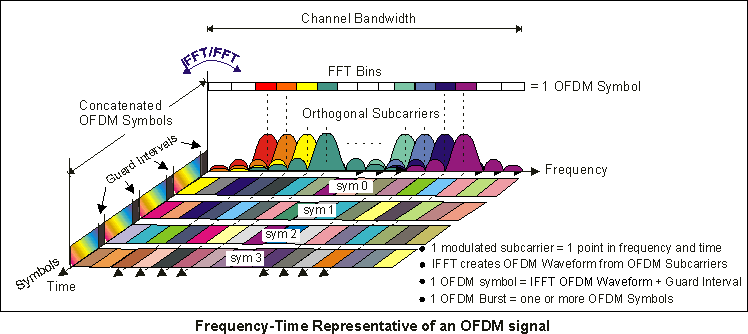
\includegraphics[width=\textwidth]{Frequence_time.png}
  \caption[Temps-Frequence]{Temps-Frequence: representation d un signal OFDM}
  \label{fig:tempsFreq}
\end{figure}

Comme nous pouvons le voir, les signaux OFDM résultent d’une modulation multi-porteuses. C’est-à-dire que nous répartissons l’information sur une bande de fréquence, autour de plusieurs porteuses de fréquences centrales également réparties. Puis, à chaque sous-fréquences porteuses, on envoie des symboles répartis dans le temps espacé par des intervalles de garde.


\paragraph{}


\newpage
%%%%%%%%%%%%%%%%%%%%%%%%

\chapter{Egalisation OFDM}
\paragraph{}

L’égalisation sert à réduire fortement, voir annuler, les interférences dues aux
multi-trajets dans le canal de propagation. Dans le domaine temporel, elle se
fait en cherchant les coefficients d’atténuation modélisant l’effet du canal.
Mais, dans le cas de transmission à haut débit, nous avons trop de recouvrement
entre symbole à cause des retards lors de la réception des différents
multi-trajets, ainsi le système devient complexe et donc le coût des terminaux
devient élevé.
\paragraph{}
L’idée de l’égalisation OFDM est de transformer l’égalisation faite dans le
domaine temporel pour un signal mono-porteuse dans le domaine fréquentiel avec
un signal multi-porteuses. Dans ce chapitre, nous décrierons tout d'abord
l'égalisation d'un point de vue théorique, pour ensuite analyser sa mise en
place pratique.


\section{Principe théorique de l'égalisation OFDM}
\paragraph{}
Nous avons un signal multi-porteuses dont la fonction de
transfert du canal de propagation n'est pas plat dans la bande passante totale
du signal.
\paragraph{}
Premièrement, plaçons nous au niveau d'une sous-porteuse. Grâce à un protocole
que nous expliquerons plus loin, nous sommes capable à cette fréquence de
déterminer la réponse du canal, c'est-à-dire le coefficient d'atténuation du
signal sur cette fréquence.
% A la fréquence de la sous-porteuse, grâce à un protocole dont nous parlerons par
% la suite, nous sommes capable de déterminer quel est la réponse du canal sur le
% signal à cette fréquence précise, c'est à dire, le coefficient d'atténuation du
% signal à cette fréquence.
Si, d'une sous-porteuse à la suivante, nous estimons être assez proche
fréquentiellement pour estimer le canal comme plat dans la bande associée à une
sous-porteuse, alors nous pouvons dire que le coefficient d'atténuation trouvé à
la fréquence de la sous-porteuse est la même dans sa bande. C'est ce que l'on
appelle être dans une zone de cohérence du canal.
\paragraph{}
Maintenant, plaçons nous à l'échelle global du signal. Nous avons plusieurs
sous-porteuses à des fréquences assez proches pour dire que la bande associée à
une porteuse est dans une zone à peu près cohérente du canal, c'est-à-dire que
par exemple, nous n'avons pas d'évanouissement soudain dans cette bande. D'après
le paragraphe précédent, nous sommes donc capable d'évaluer le coefficient
d'atténuation pour chaque bande dédiée à une sous-porteuse. Nous pouvons donc
estimer, par morceaux, la réponse fréquentielle du canal de propagation sur la
bande passante totale du signal.
\paragraph{}
Sur la Figure ~\ref{EstimPort}, on peut comprendre comment est découpée
l'estimation de la réponse fréquentielle du canal autour de chaque
sous-porteuses.

\paragraph{}
\vspace{1\baselineskip}
\begin{figure}[!h]
  \centering
  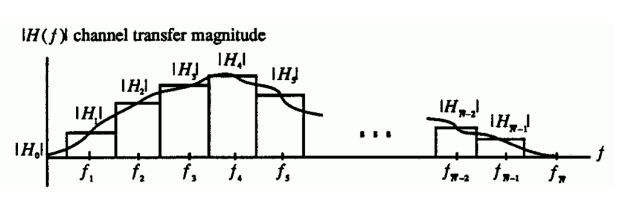
\includegraphics[width=\textwidth]{EstimCanal.png}
  \caption{Estimation du canal autour des sous-porteuses }
	\label{EstimPort}
\end{figure}

\paragraph{}
Connaissant la réponse fréquentielle du canal, nous sommes capable d'inverser
l'effet du canal après réception du signal OFDM. Le partie suivante
s'intéressera à montrer comment on estime en pratique les coefficients
d'atténuations du canal de propagation, pour ensuite décrire leur
utilisation pour inverser l'effet du canal sur le signal.


\section{Estimation pratique des coefficients d'atténuations du canal}

\paragraph{}
Le premier but de l'égalisation est d'estimer les coefficients complexes du
canal de propagation autour des fréquences des sous-porteuses. Mais la réponse
du canal de propagation varie au court du temps. Par exemple, dans un milieu
urbain, les voitures en mouvement vont réfléchir et
diffracter le signal différemment au cours du temps. Nous allons donc décrire
le protocole d'estimation de la réponse fréquentielle du canal de propagation au
cours du temps.
\paragraph{}
Ensuite, il faudra compenser l'effet du canal par calcul pour réaliser
l'égalisation. Cela est fait en prenant en compte les coefficients complexes de
la réponse fréquentielle du canal de propagation.

\subsection{Estimation des coefficients complexes}
\paragraph{}
A l'émission, nous allons insérer des valeurs constantes dédiées à l'estimation
de la réponse fréquentielle du canal. Celles-ci sont insérées avant l'IFFT, et
seront codées par une constellation connue.
%comme le chiffre 4 représente par l'état $1+j$ par exemple.
Ces valeurs, donc états, doivent être présentées sur toutes les porteuses afin
d'évaluer la réponse sur tout les canaux, même si ce n'est pas au même instant.
On doit également pouvoir répéter plusieurs fois le pilote sur chaque canal afin d'estimer
aussi la variation dans le temps de la réponse fréquentiel du canal de
propagation.

\paragraph{}
A la réception, on connaît l'état (la constellation) du pilote. On va recevoir,
avec le pilote envoyé sur la sous-porteuse n : $y_{rn}=\alpha_n.x_n+B$, avec
$y_{rn}$ le signal reçu, $\alpha_n$ le coefficient complexe la fonction de
transfert du canal à la fréquence de la sous-porteuse $n$, et donc, par zone de
cohérence, le coefficient pour la bande servant à envoyer l'état de la donnée
associée à la fréquence. $x_n$ l'état connu du pilote à l'émission. $B$
représente le bruit dans le canal de propagation. Si $\alpha_n.x_n$ est assez
grand pour que le produit $\alpha_n.x_n$ domine le bruit, on peut estimer le
coefficient complexe $\alpha_n$ par le simple calcul : $\alpha_n=y_n/x_n$. Mais
comment utiliser ce coefficient pour égaliser le signal ?

\subsection{Utilisation des coefficients complexes}
\paragraph{}
Une fois les coefficients $\alpha_n$ déterminés, nous seront capables de compenser l'effet
du canal sur le signal. Ainsi, nous aurons l'impression que la réponse
fréquentielle du canal était plate sur la bande de fréquence totale du signal
OFDM. Mais cela se fera au détriment d'une amplification du bruit.
\paragraph{}
A la réception, après démultiplexage, et calcul de la FFT sur
chaque fréquence de sous-porteuses (canaux), on divise le résultat par le
coefficient complexe avant de décoder nos états de constellation. Ce procédé est
illustré par la Figure ~\ref{UtilCoeff}.

\paragraph{}
\vspace{1\baselineskip}
\begin{figure}[!h]
  \centering
  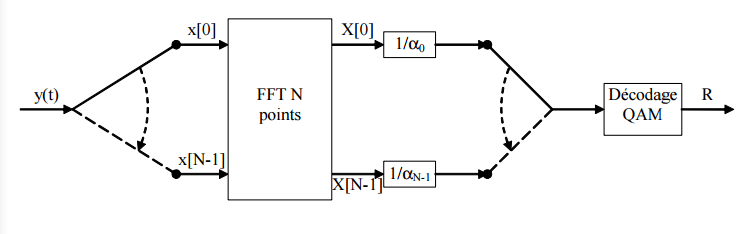
\includegraphics[width=\textwidth]{CoeffEgali.png}
  \caption{Utilisation du coefficient complexe $\alpha_n$ pour l'égalisation dans la chaine de réception }
	\label{UtilCoeff}
\end{figure}
\vspace{2\baselineskip}

\paragraph{}
Pour conclure cette partie, résumons les étapes à suivre. Afin d'estimer la
réponse fréquentielle du canal de propagation au cours du temps, nous envoyons
sur toutes les sous-porteuses, des signaux pilotes dont le codage sur un état de
constellation est connu. Nous répétons ce protocole plusieurs fois au cours du
temps afin de prendre en compte que la réponse du canal change au cours du
temps. Une fois l'estimation des coefficients effectués à la réception, nous
inversons l'effet du canal de propagation sur le signal afin d'avoir le signal
comme si la réponse fréquentielle du canal était plate sur toute la bande de
fréquence du signal OFDM. Cela est le principe de l'égalisation.

%%% Local Variables:
%%% mode: latex
%%% TeX-master: "../rapport_de_base"
%%% End:

\chapter{Rôle du préfixe cyclique dans le signal OFDM}

\section{Principe du préfixe cyclique}

Avant de répondre à cette question, nous détaillerons ici le principe d'un
préfixe cyclique et nous expliciterons sa construction. Il est à noter dans un
premier temps qu'un préfixe cyclique est un intervalle de garde
particulier. ~\\

\definition{Intervalle de garde}{Un intervalle de garde est un signal de durée
$\Delta$ que l'on place avant chaque symboles que nous souhaitons transmettre
pour réduire l'interférence inter-symboles (voir section \ref{sec:ISI}). Deux
types d'intervalles de garde sont couramment utilisés : le préfixe cyclique et
le bourrage de zéros.}

Le préfixe cyclique (souvent appelé CP) se place donc avant le symbole que l'on
souhaite transmettre. De plus le préfixe cyclique se construit comme la
répétition des derniers échantillons du bloc qu'il précède. C'est-à-dire que si
nous souhaitons transmettre $N$ état alors nous copierons $N_g$ état finaux du
symbole au début. La figure \ref{fig:PC} illustre cette copie.

\begin{figure}[!h]
  \centering
  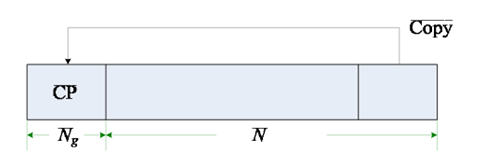
\includegraphics[width=0.7\textwidth]{pc}
  \caption{Préfixe cyclique}
  \label{fig:PC}
\end{figure}

Pour un signal OFDM, cette copie est réalisée au niveau temporelle sous chaque
sous-porteuses.

\section{Rôle du préfixe cyclique}

\subsection{Interférence inter-symboles (ISI)}
\label{sec:ISI}

\definition{Interférence inter-symboles}{\og En télécommunications, une
  interférence inter-symbole est une forme de distorsion d'un signal qui a pour
  effet que le symbole transmis auparavant affecte le symbole actuellement
  reçu\fg{}\cite{def}}




Les symboles que nous envoyons subissent des échos. Les échos correspondent aux
signal initialement envoyé mais atténué et retardé. Ils se superposent au signal
reçut de tel façon qu'a un instant $t$ il est possible de recevoir à la foi par le
signal principal le symbole $Si$ et par l'écho le symbole $S_{i-1}$: c'est l'ISI.

Si on suppose connu le temps $T_{max}$ du retard maximal d'un écho (en pratique
il est possible de déterminer les propriétés du canal), et qu'on émet un
intervalle de garde pendant un temps $\Delta > T_{max}$ alors on recevra entre
$\Delta$ et $T_s+\Delta$ uniquement le symbole $S_i$ et l'intervalle de garde
qui est connue. Une illustration est présenté à la figure
\ref{fig:intervalleGarde}.
~\\

Le préfixe cyclique étant un intervalle de garde permet de se prémunir des
interférences entre symboles (ISI).

%Il n'y a donc plus d'ISI, on est capable d'extraire facilement l'information, le
%symbole $S_{i-1}$ n'interfère plus avec le symbole $S_i$. De plus,


\begin{figure}[!h]
  \centering
  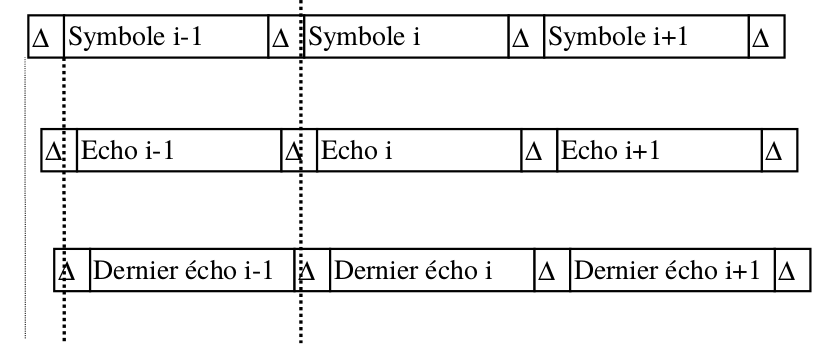
\includegraphics[width=\textwidth]{IntervalleGarde}
  \caption{Intervalle de Garde}
  \label{fig:intervalleGarde}
\end{figure}

\subsection{Interférence entre porteuses (ICI)}

\definition{Interférence entre porteuses}{Interférence dut au recouvrement des
  sous-porteuse en OFDM}

Dans ce cas ci c'est bien le caractère cyclique du préfixe qui permet d'éliminer
l'interférence entre porteuses (ICI).



%%% Local Variables:
%%% mode: latex
%%% TeX-master: "../rapport_de_base"
%%% End:


%%% Local Variables:
%%% mode: latex
%%% TeX-master: "../rapport_de_base"
%%% End:


%%% Local Variables:
%%% mode: latex
%%% TeX-master: "../rapport_de_base"
%%% End:


%%% Local Variables:
%%% mode: latex
%%% TeX-master: "../rapport_de_base"
%%% End:




%%%% CONCLUSION %%%%%%%%%

\chapter*{Conclusion}
\addcontentsline{toc}{chapter}{Conclusion}
\paragraph{}
Pour conclure, revenons sur le travail éffectué. Nous avons tout d'abord fait de nombreuses recherches bibliographique sur l'OFDM, afin d'en comprendre les principes. L'utilisation du préfixe cyclique dans les signaux OFDM permet d'éviter l'ISI et l'ICI, ce qui facilite l'estimation du canal de propagation lors de la réception. Mais le préfixe cyclique peut occuper jusqu'à 20\% du débit, auquel on ajoute encore une occupation de débit pour les pilotes permettant d'estimer le canal. Après avoir bien apréhender les spécificités de l'OFDM, nous nous sommes intéressés à l'extraction du préfixe cyclique afin de monter en débit. Sans ce préfixe, nous avons de l'ICI qui apparait, ce qui complique fortement l'étape d'égalisation. En comprenant le rapport scientifique \cite{sujet} en annexe à la page \pageref{annexe}, nous avons tout d'abord mis en évidence, grâce à Matlab, la réussite des structures d'égalisation DFVE (temporelle et fréquentielle) en éstimant connaître le canal de propagration. Mais en réalité, la réponse fréquentielle du canal change, et nous ne le connaissons pas. Nous avons donc ajouté des pilotes à notre signal à l'émission, afin d'éstimer le canal à la réception. Grâce à l'algorithme LMS, nous avons réussi à faire converger l'éstimation du canal vers la bonne réponse fréquentielle. 






\newpage

%%%% ANNEXE %%%%%%%%%%%%

\part*{Annexe}
\label{annexe}
\appendix
\nocite{*}
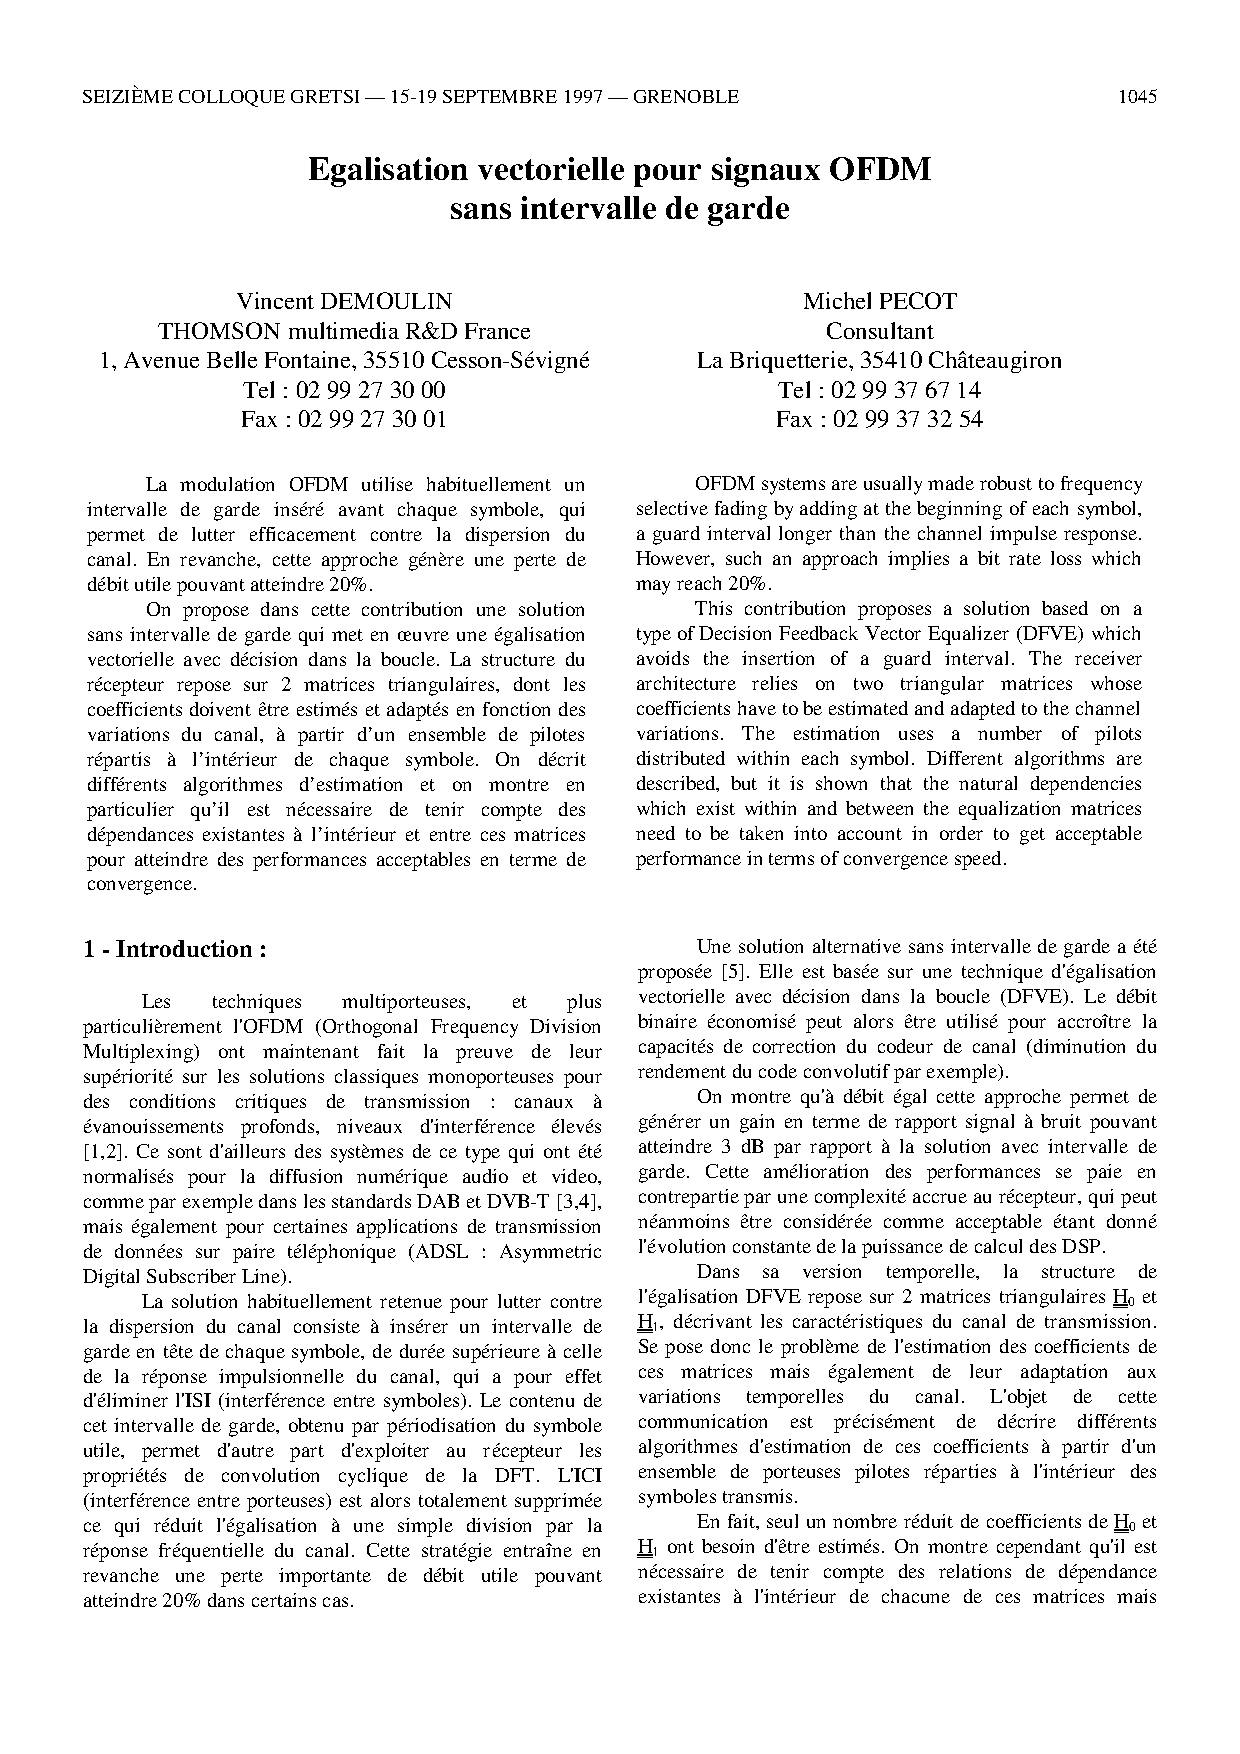
\includepdf[pages=1-4]{./../ressource/261_373.pdf}
\newpage
 \listoffigures
 \printindex
 \bibliographystyle{frplain}
  \bibliography{biblio}

\end{document}
%%%%%%%%%%%%%%%%% FIN DU DOCUMENT
%%% Local Variables:
%%% mode: latex
%%% TeX-master: t
%%% End:
